\documentclass[10.5pt]{article}
\usepackage[shortlabels]{enumitem}
\usepackage[a4paper, total={6in, 8in}]{geometry}
% multicolumn text
\usepackage{multicol}
% wrapfigures
\usepackage{wrapfig}
% hyperlinks
\usepackage{hyperref}
% frames around texts
\usepackage[framemethod=tikz, xcolor=true]{mdframed}
% filler text
\usepackage{blindtext}
% code einbetten und konfigurieren
\usepackage{listings}
% referencing with names
\usepackage{nameref}
\usepackage{xcolor}
\usepackage{fancyhdr}
\usepackage{amsfonts}
\usepackage{amsmath}
\usepackage{stmaryrd}
\usepackage{titling}
% zitieren
\usepackage{cite}
% Graphics
\usepackage{graphicx}
\graphicspath{ {./figures/} }

%rote Frames für Hinweise
\newenvironment{attention}{\begin{mdframed}[tikzsetting={draw=red, thick}]\textbf{Attention:} \\}{\end{mdframed}}
%blaue Frames für Formeln
% \newenvironment{blueframe}{\begin{mdframed}[tikzsetting={draw=blue, thick}]}{\end{mdframed}}

\author{Luik Fischer}
\title{Rubrics Tool Benutzeranleitung und Hinweise}

% fancyhdr setup
\pagestyle{fancy}
\lhead{}
\cfoot{}
\rfoot{Seite \thepage}
\renewcommand{\headrulewidth}{0.5pt}
\renewcommand{\footrulewidth}{0.5pt}

\begin{document}

% \maketitle
% \tableofcontents
% \newpage

\section{General}
\label{sec:general}
Using the \textit{Rubric Tool} involves two jobs:

\begin{enumerate}
  \item \textbf{Creating Tasks} \\
    For each task (i.e., an assignment, project, or any other gradeable task), a new task should be created by clicking \textit{Create New Task} on the \textit{Home Screen}. Meta-information concerning this task can be entered here and then saved to your personal task list, or exported and downloaded as a JSON-File.
  \item \textbf{Assess Solutions} \\
    The people who assess the tasks (i.e. tutors) can use the JSON-File created in the previous step to do so. They can select a task from the list in their \textit{Home Menu} and press \textit{Fill out Rubric} to assess the solutions according to the task structure defined in \textbf{Creating Tasks}. Within the assessment step they can work on different students solutions consecutively and export the results of their assessment as a \textit{CSV}- or \textit{JSON}-File.
\end{enumerate}

\begin{attention}
  The current progress of an \textit{assessment session} or a \textit{task creation session} is only persisted in the \textit{local storage} of the web page. This storage instance is wiped when the browser history is cleared or the local storage is wiped specifically. Further details on persistence are discussed in the chapters \nameref{sec:taskcreation} and \nameref{sec:assessment}.
\end{attention}

The full implementation of the tool can be found on \href{https://github.com/0nlineSam/rubrics-creation-tool}{https://github.com/0nlineSam/rubrics-creation-tool}.

\section{Home Screen}
\label{sec:home}
The \textit{Home Screen} is the entry point to the web application (siehe Figure~\ref{fig:homescreen}).
From here the user can \textit{upload an existing task} (label 1), \textit{create a new task} (label 2), \textit{see a list of saved tasks} (label 3) and \textit{fill out a rubric} (label 4). The labels are further described below.

\begin{itemize}
  \item[\textbf{1:}] The user can upload a \textit{task}, a JSON-File in order to fill out the rubric.
  \item[\textbf{2:}] The user can create an entirely new \textit{task}.
  \item[\textbf{3:}] The user can view a list of \textit{tasks} available for assessment.
  \item[\textbf{4:}] The user can start the \textit{assessment process} and fill out an existing task.
\end{itemize}

\begin{figure}[h]
  \begin{center}
    
\includegraphics[width=0.9\textwidth]{figures/homescreen}
  \end{center}
  \caption{Screenshot of the \nameref{sec:home}}
  \label{fig:homescreen}
\end{figure}


\section{Creating Tasks}
\label{sec:taskcreation}
\subsection{Granularity}
The granularity of a \textit{task} is defined by the lecturer (or creator of the task). At the coarsest granularity in the context of, for example, exercise sheets, a \textit{task} should reflect one exercise sheet. Of course a finer level of granularity can be chosen. In the context of exercise sheets this could mean, that there is one \textit{task} per task on an exercise sheet. Ultimately it is the lecturers responsibility to communicate the granularity of the \textit{task}.

\subsection{Process of Task Creation}
The process of \textit{task creation} is designed in a linear fashion. There are four consecutive steps involved in \textit{task creation}.

\begin{enumerate}
  \item Entering general information. Part of the \nameref{sub:metainfo}.
  \item Selecting a main topic. Part of the \nameref{sub:metainfo}.
  \item Selecting \nameref{sub:features} with their associated \textit{weights}.
  \item Overviewing and validating the choices made in the previous steps.
\end{enumerate}

In order to get to the next/previous step the user can press the \textit{BACK}-/\textit{NEXT}-Buttons (labeled 9 and 10 in Figure~\ref{fig:taskcreation1}).

\subsection{Meta-Information}
\label{sub:metainfo}
Specifying the meta-information for a \textit{task} is done by clicking the \textit{"Create New Task"}-Button on the \nameref{sec:home}.
The steps 1 and 2 are desgined to enter this meta-information consisting of the following parameters (marked with corresponding labels 
in Figure~\ref{fig:taskcreation1} and Figure~\ref{fig:taskcreation2}):

\begin{enumerate}
  \item \textbf{Course} \\
    Select the couse to which the assignment belongs. A dropdown provides a list of available courses.
  \item \textbf{Task Name} \\
    A name for the task. This name should \textbf{not} be empty and has to be \textbf{unique} in order to \textit{add the task} to the home screen list (Figure~\ref{fig:homescreen}, label 3). The name does not have to be unique in order to export the task as a JSON-File.
    \begin{attention}
      Only use \textbf{characters} that are \textbf{legal in file names}. The \textit{name} will be part of the exported file name.
    \end{attention}
  \item \textbf{Task Week} \\
    The week in which the task has to be solved. Also indicates the expected knowledge level of the students.
  \item \textbf{Max Points} \\
    Specify the maximum number of points that students can achieve in this \textit{task}. This is also used for computation of the final score achieved by the student, when the \textit{rubric} gets \textit{filled out}.
  \item \textbf{Differentiation of Background} \\
    Only change this value if the course is a \textit{TU/e}-course. This value corresponds to different variants of assignments.
  \item \textbf{QPED Deliverables} \\
    Select all QPED deliverables that students have used for this assignment. Either because they were used to teach the topics that are practiced by this assignment, the assignment itself uses a deliverable or students may use a deliverable to solve the assignment. 
  \item \textbf{Task Description} \\
    Used to provide a short description of the task at hand. The main purpose of this parameter is to allow the assessors of a \textit{task} to quickly verify that they are assessing the right \textit{task}.
  \item \textbf{Main Topic} \\
    Select a main topic for the \textit{task}. The available topics are nested within categories. This \textit{main topic tree} is depicted as a dropdown. In order to select a topic, you have to select a \textit{leaf node} of this tree.

\end{enumerate}

\begin{figure}[h]
  \begin{center}
    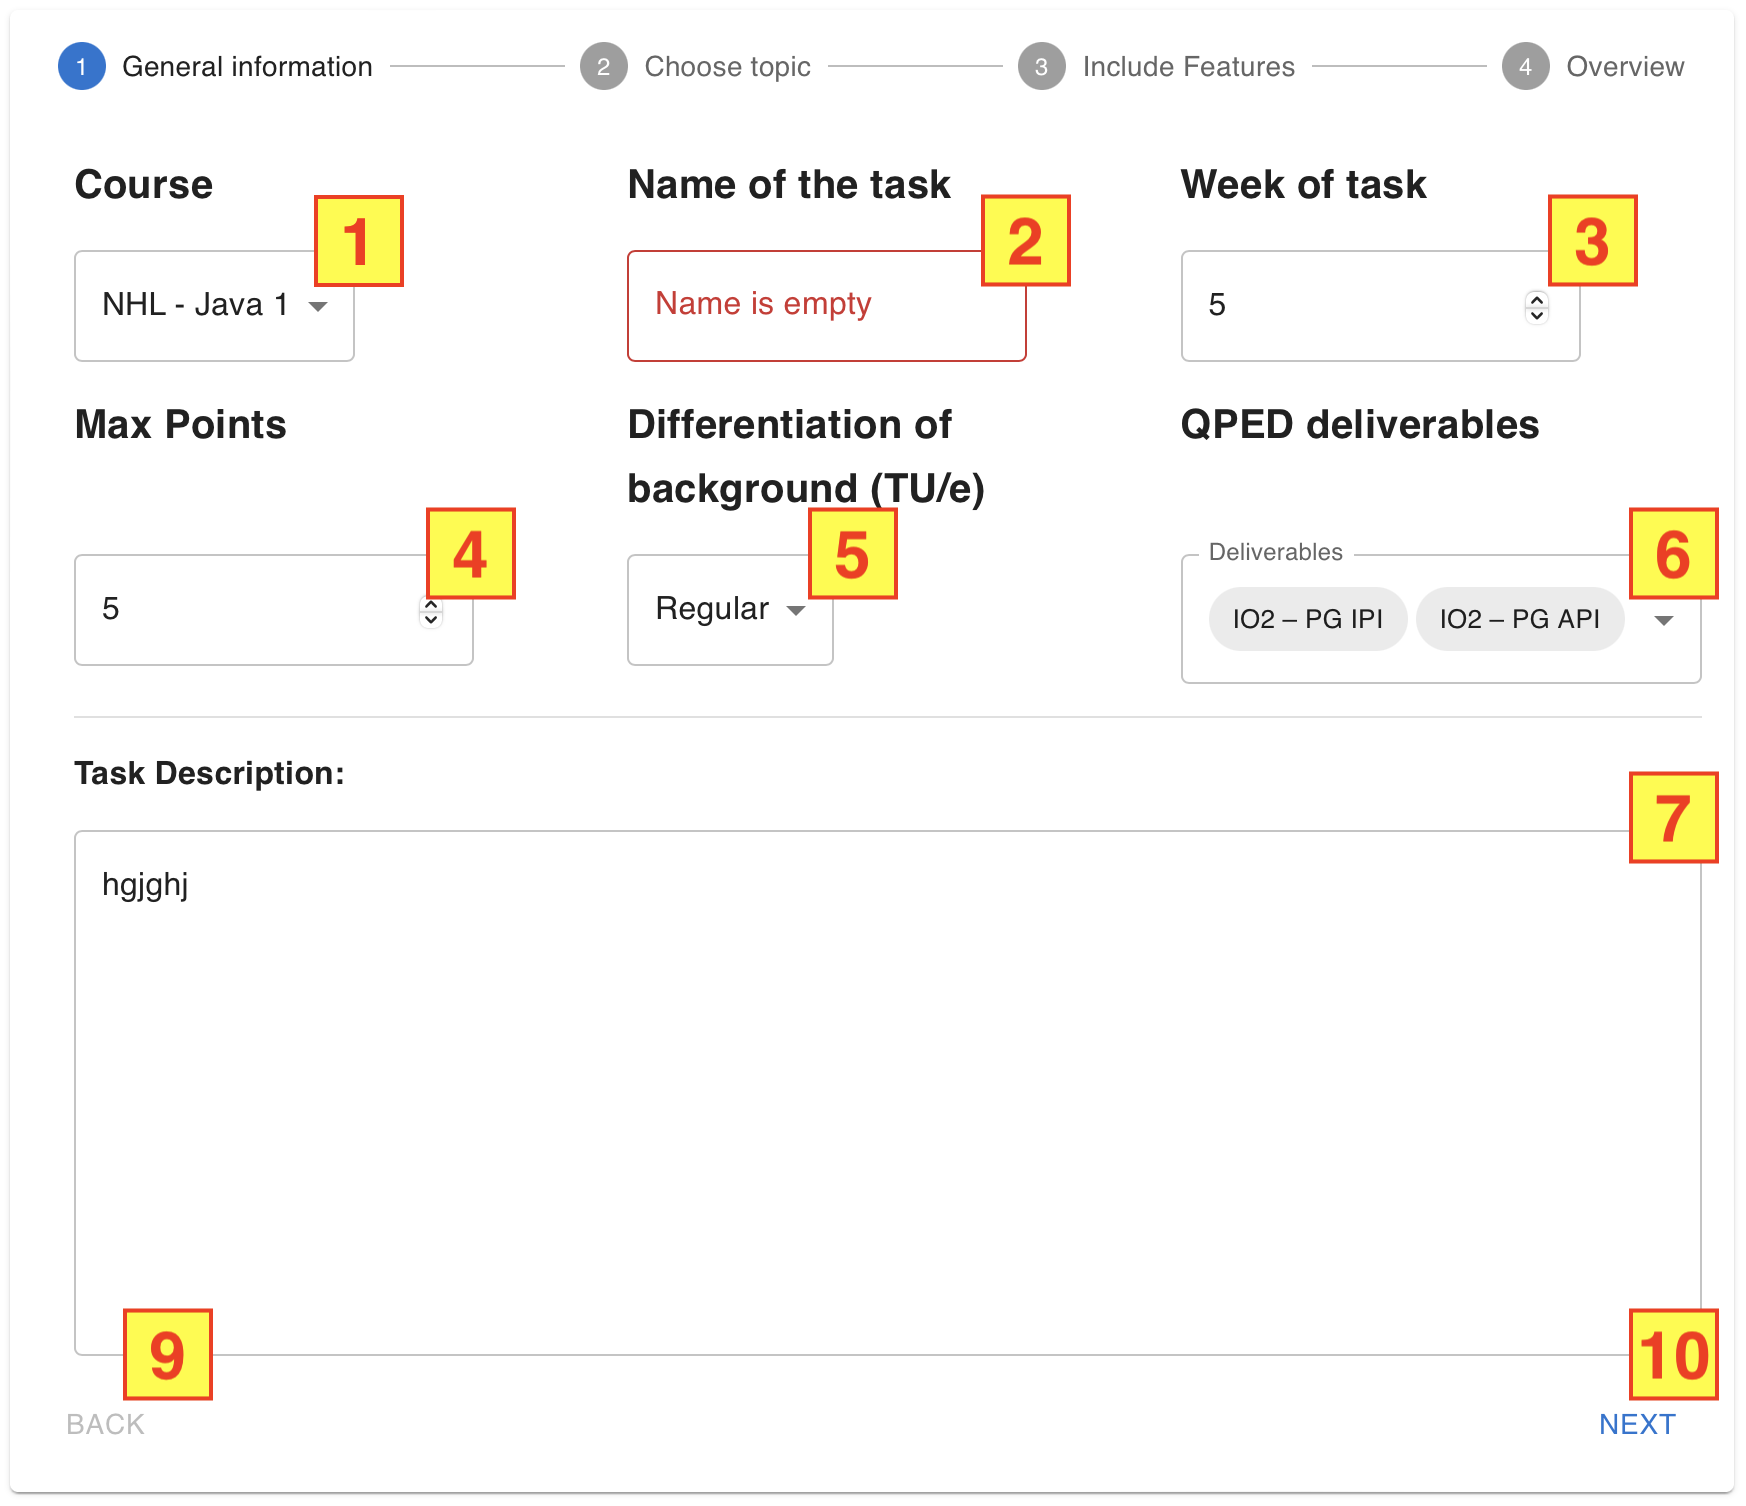
\includegraphics[width=0.95\textwidth]{figures/taskcreation1}
  \end{center}
  \caption{Step one of the \textit{task creation process}.}
  \label{fig:taskcreation1}
\end{figure}

\begin{figure}[h]
  \begin{center}
    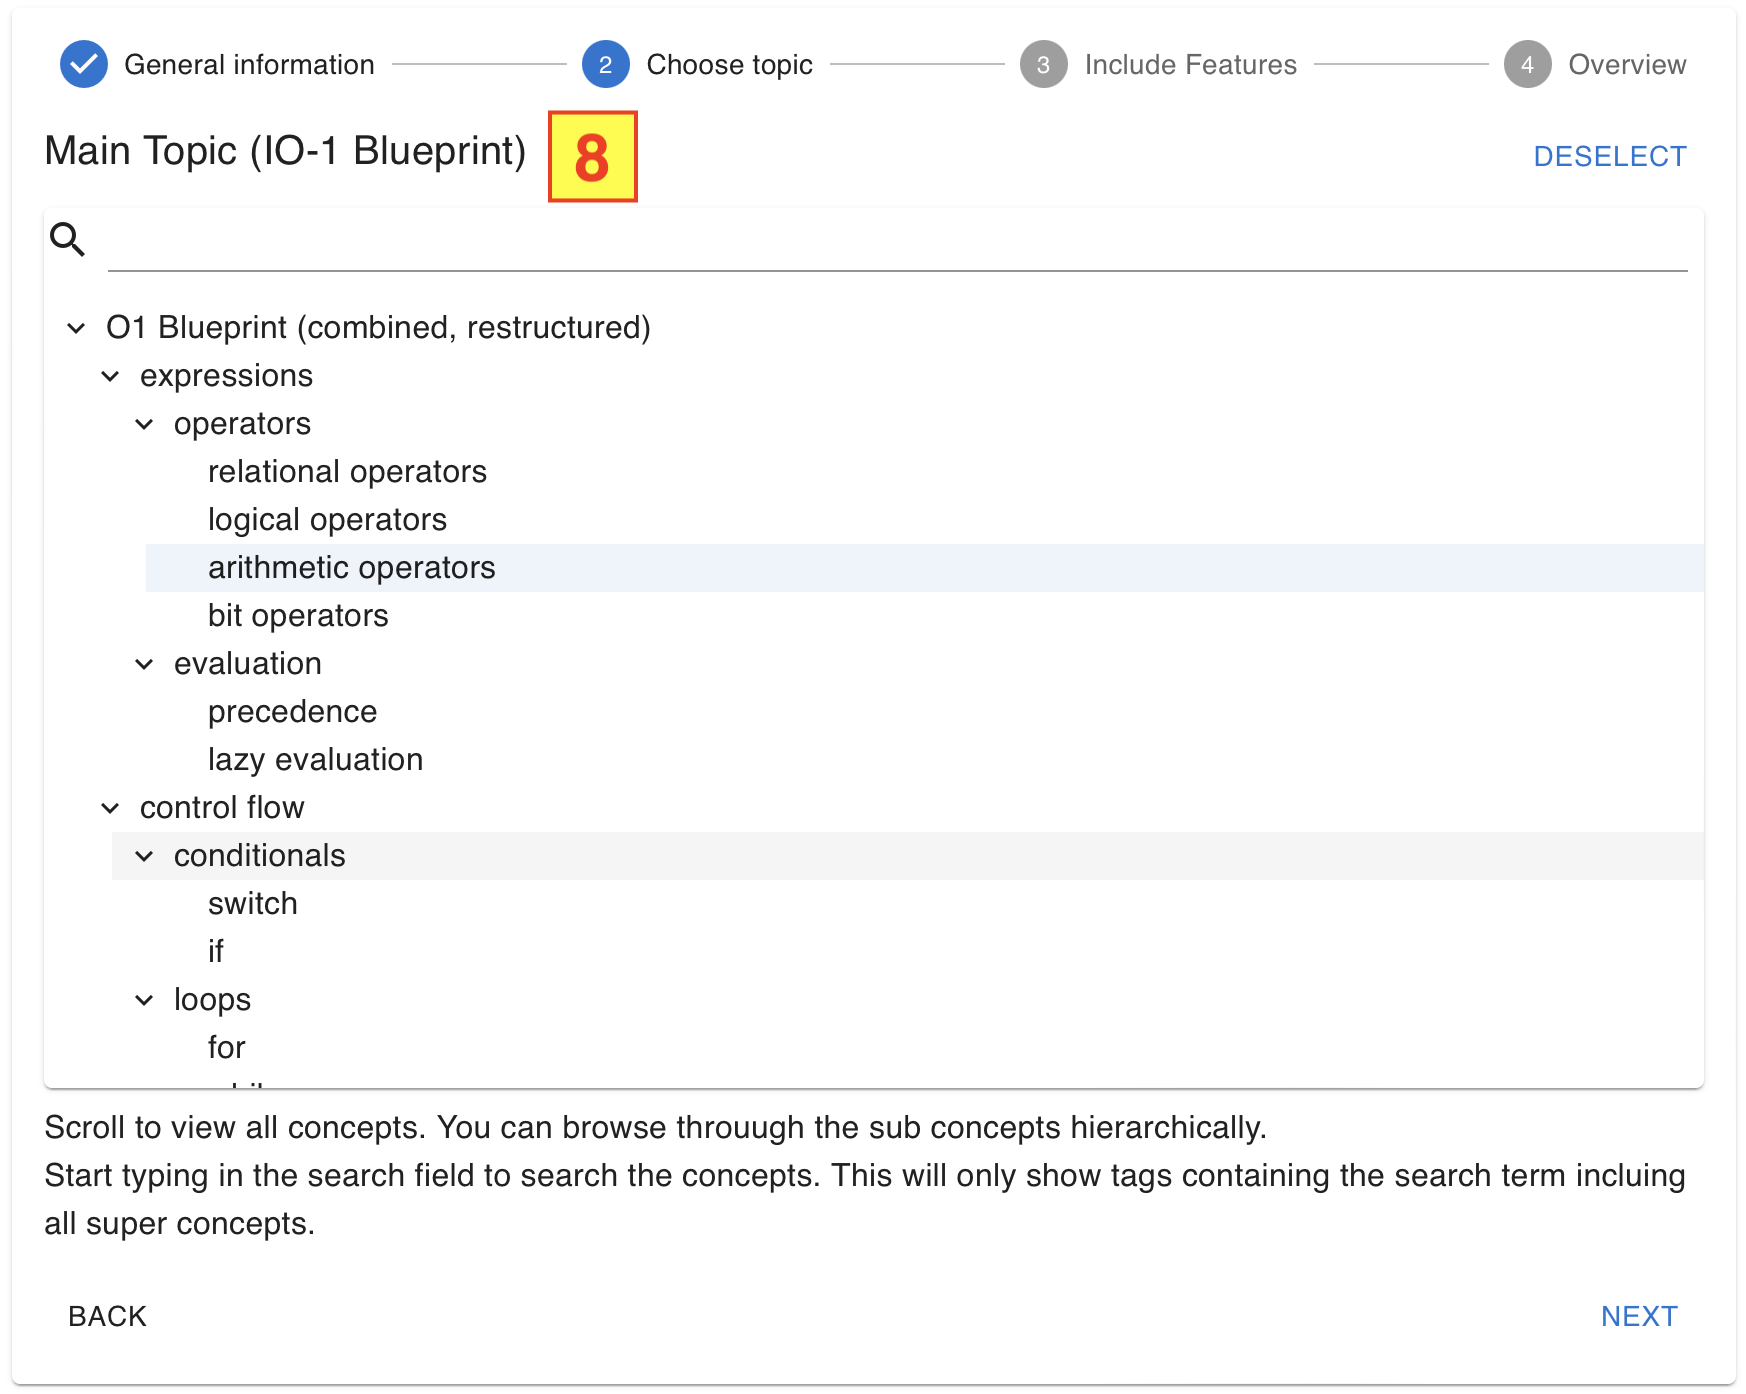
\includegraphics[width=0.95\textwidth]{figures/taskcreation2}
  \end{center}
  \caption{Step two of the \textit{task creation process}.}
  \label{fig:taskcreation2}
\end{figure}


\subsection{Features}
\label{sub:features}
Features for a \textit{task} can be selected from three main groups: \textit{Basic}, \textit{Advanced} and \textit{Procedural Guidance}.
Set a check to include the corresponding feature and chose a weight to determine how heavily the students ability to fulfill this requirement affects the score.

\section{Assessment of solutions}
\label{sec:assessment}
\input{chapters/4assessment.tex}
\section{Personal Settings}
\label{sec:settings}
\input{chapters/5settings.tex}

\newpage

\end{document}
